\chapter{Event and Population Analysis}\label{ch:analysis}

    Using the population models described in Chapter \ref{ch:synthesis}, one can derive
    the properties of NSBH mergers as seen in the GW and EM regimes.
    Specifically, an important aspect of NSBH mergers is what fraction of mergers
    actually produce a prompt component which will be detectable by present-day
    gamma-ray detectors, such as INTEGRAL. A related aspect is the dependence of this
    fraction on the priors which go into creating these populations. Specifically,
    different black hole spin prior distributions would affect the number of detectable
    prompt emissions, and so this behaviour is worth investigating. Furthermore, this
    population synthesis framework may also help to investigate the rate density of NSBH
    mergers which lead to observable SGRBs, which can then be compared to the rate
    derived currently from purely EM observations.\\
    Additionally, events seen solely in the GW regime without any confident EM
    counterparts may be analysed using the framework set up here. Using the posterior
    distributions for the component masses, spins etc., derived from GW strain data
    analysis, one can derive the corresponding remnant, dynamic and disc masses from
    which the jet energetics can be derived. Under the assumptions of the underlying
    model, this process of computation can then help eliminate or give credence to the
    existence of EM counterparts for events observed via GW only.

\section{Analysis of Population Synthesis Models}

    From the description of the population models given in Chapter \ref{ch:synthesis},
    it is clear that there are three classes of populations, segregated by the black
    hole spin population that is used. Specifically, the three classes of populations
    are:

    \begin{itemize}

        \item \textbf{Class I} -- this uses the standard \textsc{truncated} BH mass
            distribution with a contant NS mass of 1.4 M$_\odot$. The BH spin
            distribution is the beta distribution from \cite{abbott_2020B}, and the NS
            spin is set identically to 0 for all samples (see \S\ref{sec:ns_pop}
            for reasons on why this assumption is valid). The remaining NS parameters
            and their computation (such as the NS compactness, tidal deformability etc.)
            are described in \S\ref{sec:ns_pop}, and thus omitted for brevity.

        \item \textbf{Class II} -- here, the BH spin distribution is assumed to be
            uniform between [0, 1). The rest of the binary parameter distributions are
            the same as in Class I.

        \item \textbf{Class III} -- here, the BH spin is a "restricted" Gaussian
            distribution between [0, 1), which means that samples between [0, 1) are
            taken as is but samples outside of this range are discarded.  For the
            purposes of being general, samples are drawn from distributions with stanard
            deviation, $\sigma = 0.2$ and mean, $\mu = 0.2, 0.5, 0.7$.  The rest of the
            binary parameter distributions are the same as in classes I and II.

    \end{itemize}

    For each population, 10$^5$ samples are drawn from the relevant populations. Using
    the samples, the various mass parameters required to compute the energetics of the
    jet are calculated using Eqs. \ref{eq:m_out} -- \ref{eq:constraint}. Then, using Eq.
    \ref{eq:e_kin_jet} -- \ref{eq:eiso}, the jet structure is imposed and for each event
    the value of $E_{iso}(\theta_v)$ is computed. These are then converted into fluences
    using the equation:

    \begin{equation}
        \mathcal{F} = \dfrac{E_{iso}(\theta_v)}{4\pi d_L^2}
    \end{equation}

    This is done in order to ascertain the detectability of the prompt emission, with a
    typical gamma-ray detector, such as the INTEGRAL satellite, as a reference. The
    INTEGRAL satellite has a lower fluence cutoff of $2 \times 10^{-7}$ erg, and so with
    respect to this detector, any event with a fluence lower than this value will be
    considered a non-detection. Albeit this is a tight and somewhat ephemeral
    restriction, it helps to ascertain the rough number of detections versus
    non-detections.\\
    Similarly, with the binary parameters set by the sampling process, the GW network
    SNR is computed with the RWF as the GW template, using Eqs. \ref{eq:rho} --
    \ref{eq:freq_integral}. The detector network configuration consisting of Advanced
    LIGO (LIGO-Livingston, L1 and LIGO-Hanford, H1) and VIRGO (V1) detectors was set up
    using PyCBC's \texttt{detector} module, which builds up the detector locations,
    antenna pattern functions, location phase factors etc. For all three detectors, the
    Advanced LIGO Design sensitivity was used as an approximation for their respective
    future configurations. This was done, since with the current network configuration,
    there have been no confident detections of NSBH mergers which have \textit{also} had
    an EM counterpart.\\
    The results of the simulations are given below, with each population producing a
    particular number of NSBH binary merger events seen in:

    \begin{enumerate}

        \item The GW regime alone, $\boxed{\mathcal{N}_{GW}}$ -- these are events whose
            GW network SNR is calculated to be higher than the network SNR threshold of
            10.

        \item The EM regime alone, $\boxed{\mathcal{N}_{EM}}$ -- these are events whose
            simulated gamma-ray fluence is calculated to be above the INTEGRAL fluence
            limit of $2 \times 10^{-7}$ erg.

        \item The GW \textit{and} EM regimes both, $\boxed{\mathcal{N}_{EM+GW}}$ --
            these are events which satisfy both the GW and EM `cutoffs', and thus
            represent joint detections.

    \end{enumerate}

    These numbers are collected together in Table \ref{tab:popln_numbers} for each
    population class. From this table it is evident that the spin distribution heavily
    affects the number of EM-only events, and by extension the number of joint events.\\
    This can be explained by looking at the dependence of $M_{disc}$ on the BH
    spin, from Eq.\ref{eq:disc_mass}, for a fixed mass ratio. Since a highly spinning
    black hole produces more tidally disrupted material for a given mass ratio than a
    low spinning black hole, binaries with a higher black hole spin are more likely to
    produce a more massive disc (assuming not much mass is lost as dynamical mass).
    This behaviour of $M_{disc}$ is also shown below in Fig. \ref{fig:m_disc}.

    \begin{table}[H]
        \centering
        \caption{Number and Kind of Detections across Population Classes}
        \begin{tabular}{cccc}
            \toprule

                &
            $\mathcal{N}_{GW}$ &
            $\mathcal{N}_{EM}$ &
            $\mathcal{N}_{EM+GW}$ \\

            Class I & 26 & 12283 & 0 \\

            Class II & 640 & 12283 & 88 \\

            Class III$_{\mu = 0.2}$ &
            19 & 12283 & 0 \\
            Class III$_{\mu = 0.5}$ &
            266 & 12283 & 26 \\
            Class III$_{\mu = 0.7}$ &
            882 & 12283 & 118 \\
            \bottomrule
        \end{tabular}
        \label{tab:popln_numbers}
    \end{table}


    \begin{figure}[H]
        \centering
        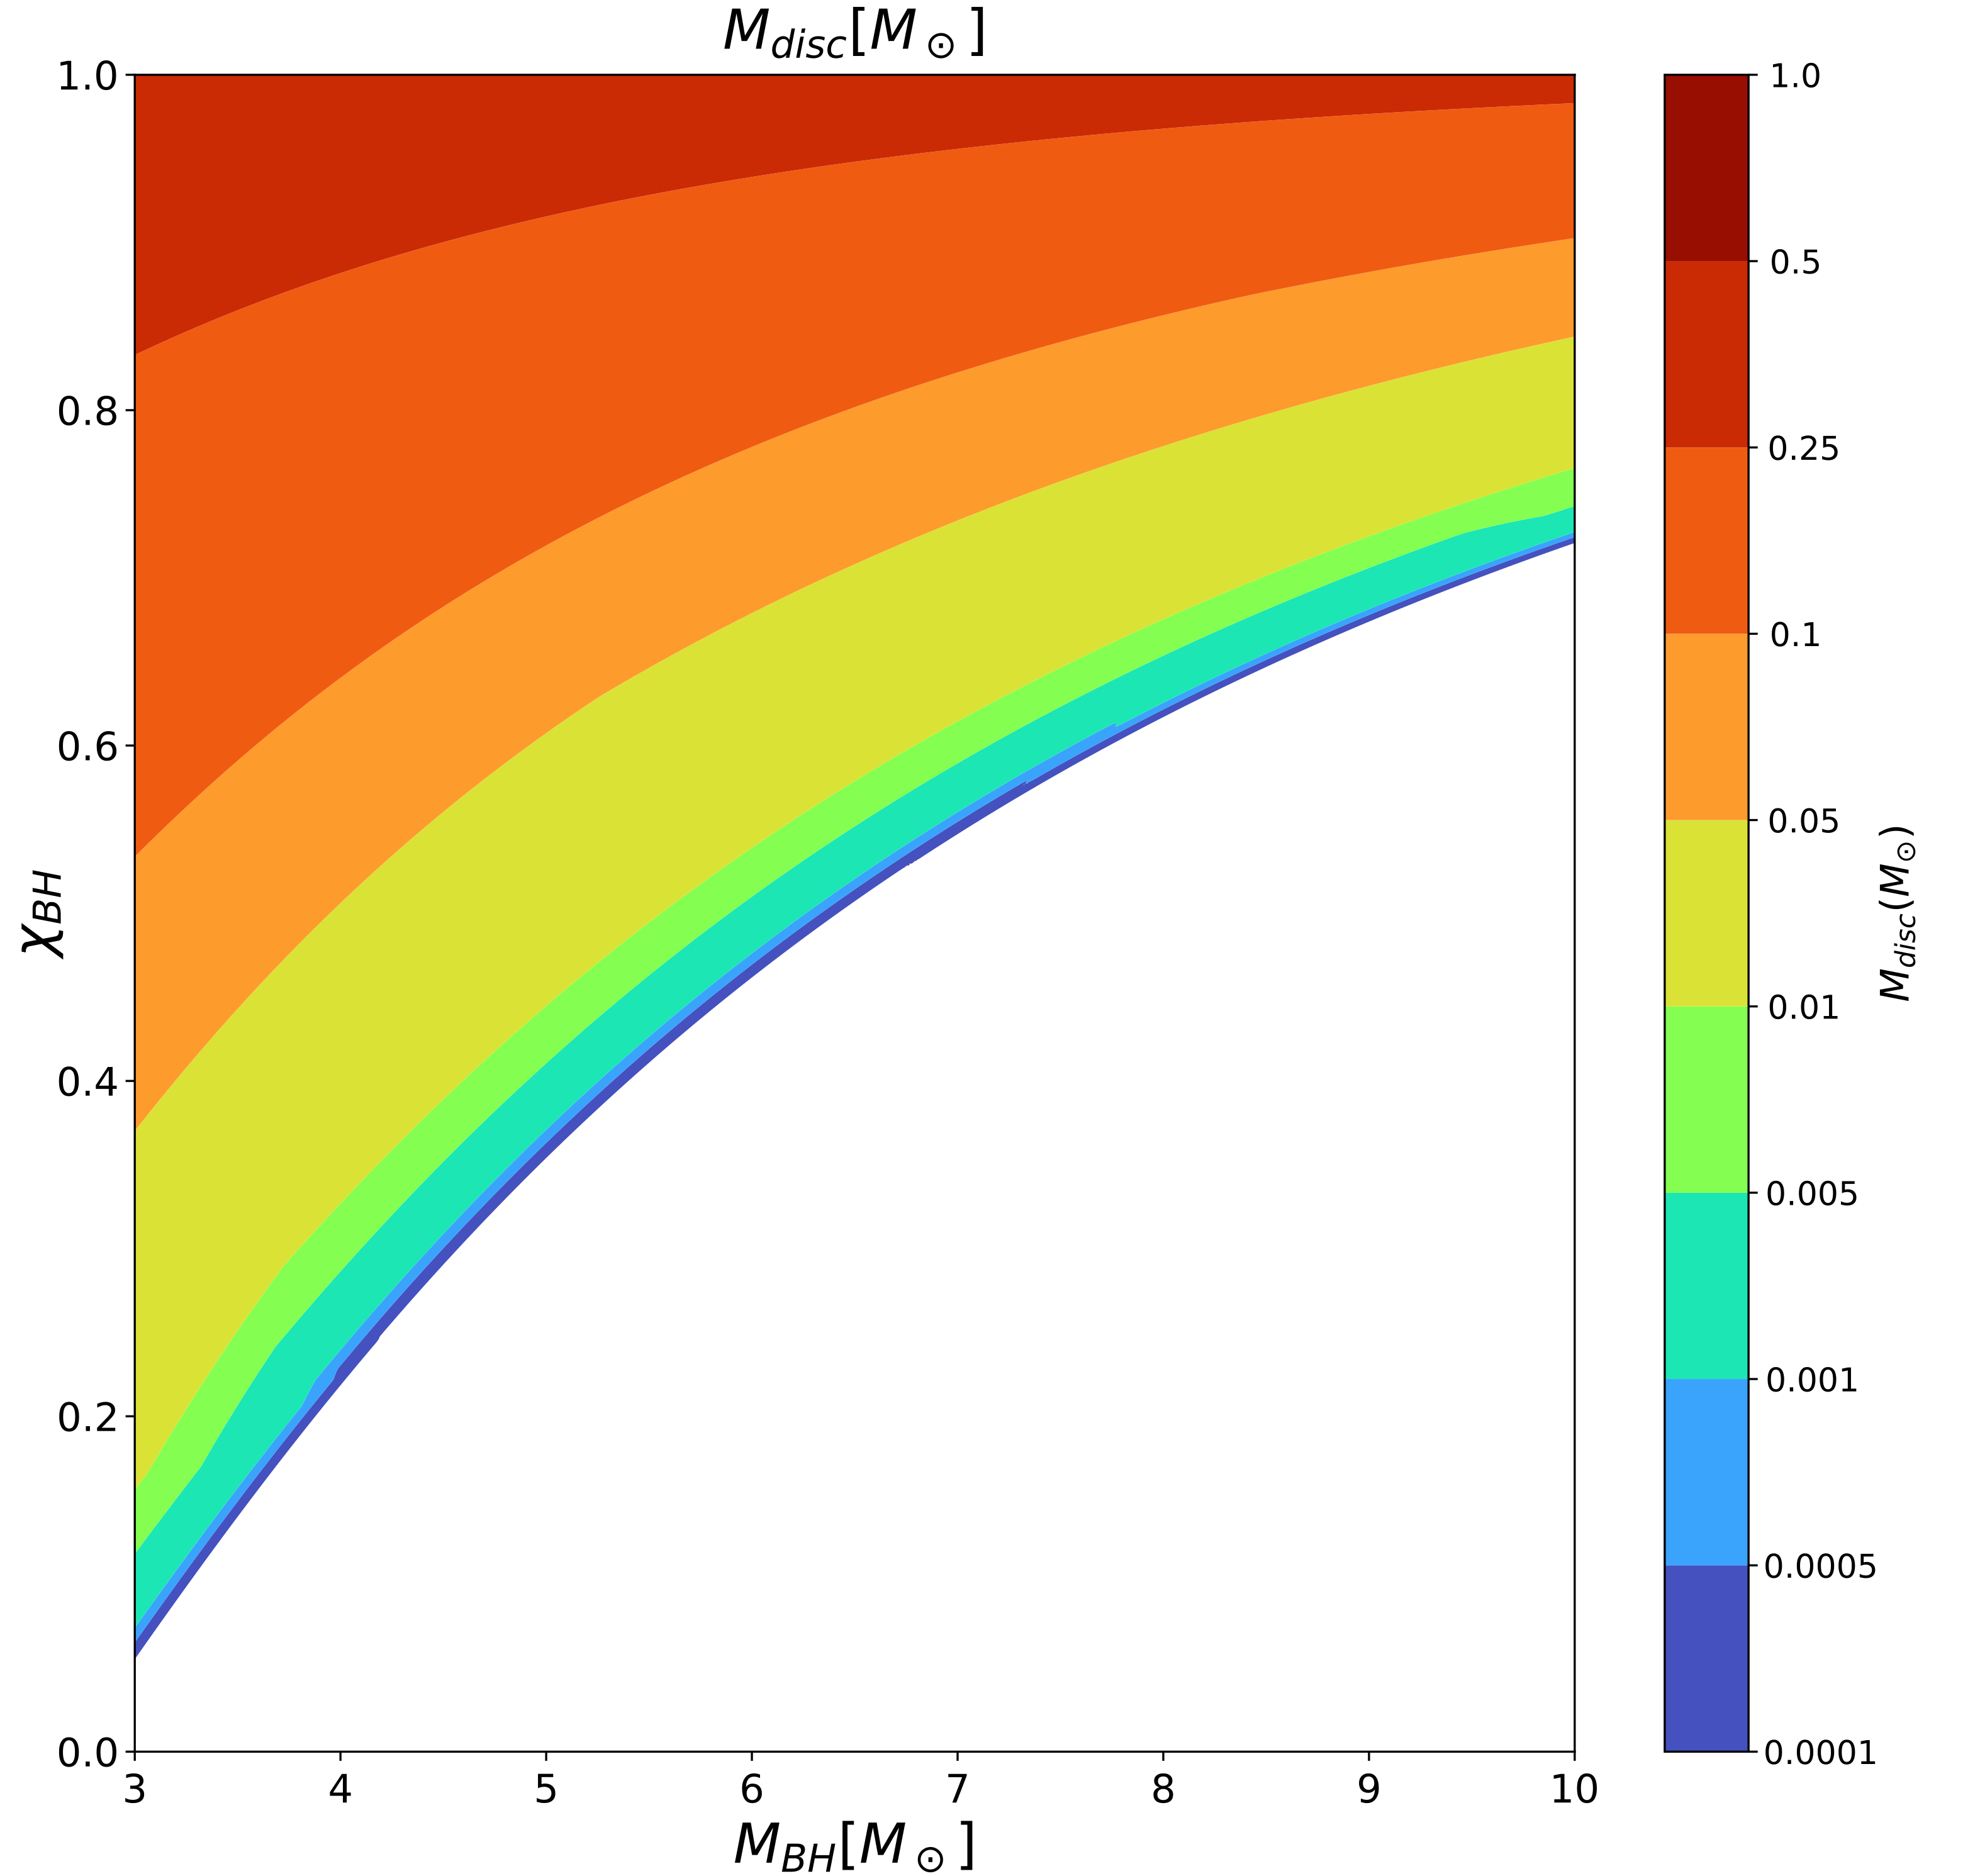
\includegraphics[width=0.8\linewidth]{m_disc}
        \caption[Variation of $M_{\mathrm{disc}}$ with $\chi_{BH}$ and $\mathcal{Q}$]{
            Variation of the disc mass with the mass ratio, $\mathcal{Q}$ and the black
            hole spin, $\chi_{BH}$. Note that the higher disc mass values are achieved
            when $\chi_{BH}$ is high and $\mathcal{Q}$ is low. Reproduced from
            \cite{barbieri_2019b}.
        }
        \label{fig:m_disc}
    \end{figure}

    This then means that because populations with igh spin' distributions (such as
    Class I or Class III$_{\mu = 0.7}$) have a higher proportion of high spin binaries,
    they have a higher number of EM and joint detections, since a more massive disc
    produces a more energetic jet from Eq.\ref{eq:eiso}, and thus increases the
    possibility of detections.

\section{Event Analysis}\label{sec:event_analysis}

    \subsection{GW190426\_152155}\label{ssec:nsbh_190426}

        This event, as described in GWTC-2 and in \S\ref{sec:190426}, has an
        astronomical source probability of 42\% and a terrestrial event possibility of
        ~52\%. Even though this is the case, there is still speculation on whether this
        event could be an NS merger event.  This is still possible since the priors used
        for the classification mechanism depend sensitively on knowledge about the
        stocastic GW background and the source classification may very well change in
        the future, as more analysis is done on the GW noise observed as the LIGO/VIRGO
        interferometers operate.\\
        With this uncertainty in mind, asking the question of whether GW190426\_152155
        could be an NSBH event is pertinent, and the current framework makes for a
        suitable test bed to test this hypothesis with. Using the LSC data release for
        the binary system parameters associated with GW190426\_152155, which gives
        samples from the posterior distributions for $M_{BH}, M_{NS}$ etc., the disc
        mass was computed for each set of binary parameters. Computing the disc mass is
        expeditious since it directly gives an estimate of how many sets of samples will
        be able to \textit{atleast launch} a jet, since if $M_{disc} = 0$ for a
        particular set of samples, there is no possibility of detecting a jet from this
        particular binary.\\
        Fig. \ref{fig:mdisc_q_190426} is the result of this analysis in the
        $\chi_{BH}-\mathcal{Q}$ plane. From that figure, it is seen that a very small
        fraction of posterior samples actually fall within the section of the parameter
        space where $M_{disc} \neq 0$. This means correspondingly that the
        probability of the NSBH event GW190426 launching a SGRB jet at all is very low.
        This can be interpreted trivially to conclude that the event was of terrestrial
        origin, and thus it follows that it would not be compatible with the launching
        of an astrophysical jet. But non-trivially, one can also conclude that one of
        the following is true:

        \begin{itemize}

            \item The event GW190426 was a BNS merger event, which had a jet that was
                launched via other mechanisms.

            \item The event GW190426 was an NSBH merger event, but the jet was launched
                via a mechanism that is unknown. This means that the current analysis is
                invalid, and the true nature of the jet launching mechanism is unknown.

        \end{itemize}

        The actual non-detection of such a jet (if launched under these alternative
        conditions) could be either due to the inefficiency of the internal engine of
        such alternative jet launching mechanisms, or due to a viewing angle large
        enough that the jet was relativistically deboosted to below the thresholds of
        current-day gamma-ray observatories.

        \begin{figure}[H]
            \centering
            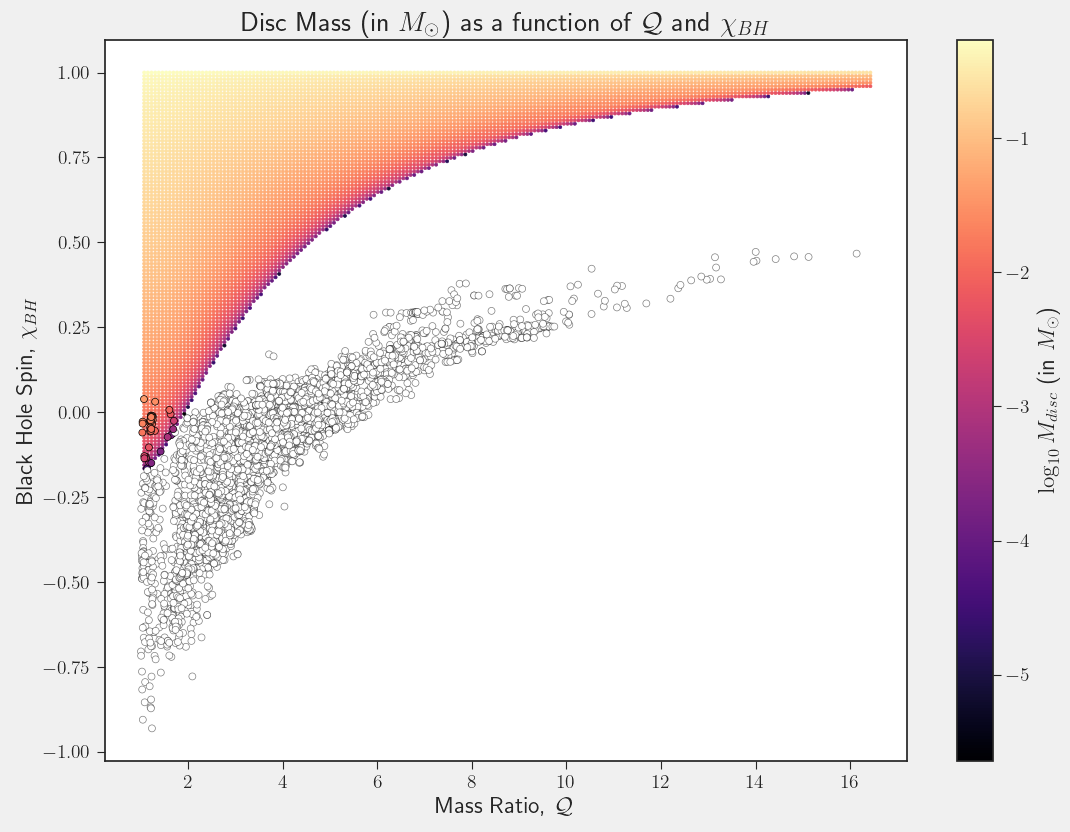
\includegraphics[width=0.9\linewidth]{mdisc_q_190426}
            \caption[GW190426 in the $\chi_{BH}-\mathcal{Q}$ plane]
            {
                GW190426 in the $\chi_{BH}-\mathcal{Q}$ plane. The color coding at a
                point in the plane indicates the value of $M_{disc}$
                corresponding to that particular $\chi_{BH}$ and $\mathcal{Q}$.
                Unfilled circles with a black outline correspond to samples from the
                posterior distributions for GW190426, which have $M_{disc} =
                0$, and so cannot support jet launching, and filled black circles are
                those with $M_{disc} \neq 0$.
            }
            \label{fig:mdisc_q_190426}
        \end{figure}

    \subsection{GW170817}

        For GW170817, as described in Chapter \ref{ch:introduction}, a lot of questions
        remain regarding the specifics of the jet launching mechanisms. Recent studies
        also show that there is a non-negligible possibility that the event was an NSBH
        merger, with a low mass BH acting as the other, non-NS component (see for
        example, \cite{hinderer_2019}). This would be compatible with the outflows
        observed from GW170817, specifically the SGRB jet GRB170817A, optical Kilonova
        AT2017gfo and associated afterglows (see \cite{abbott_2017}) since NSBH mergers
        also can produce similar outflows as shown below.

        \begin{figure}[H]
            \centering
            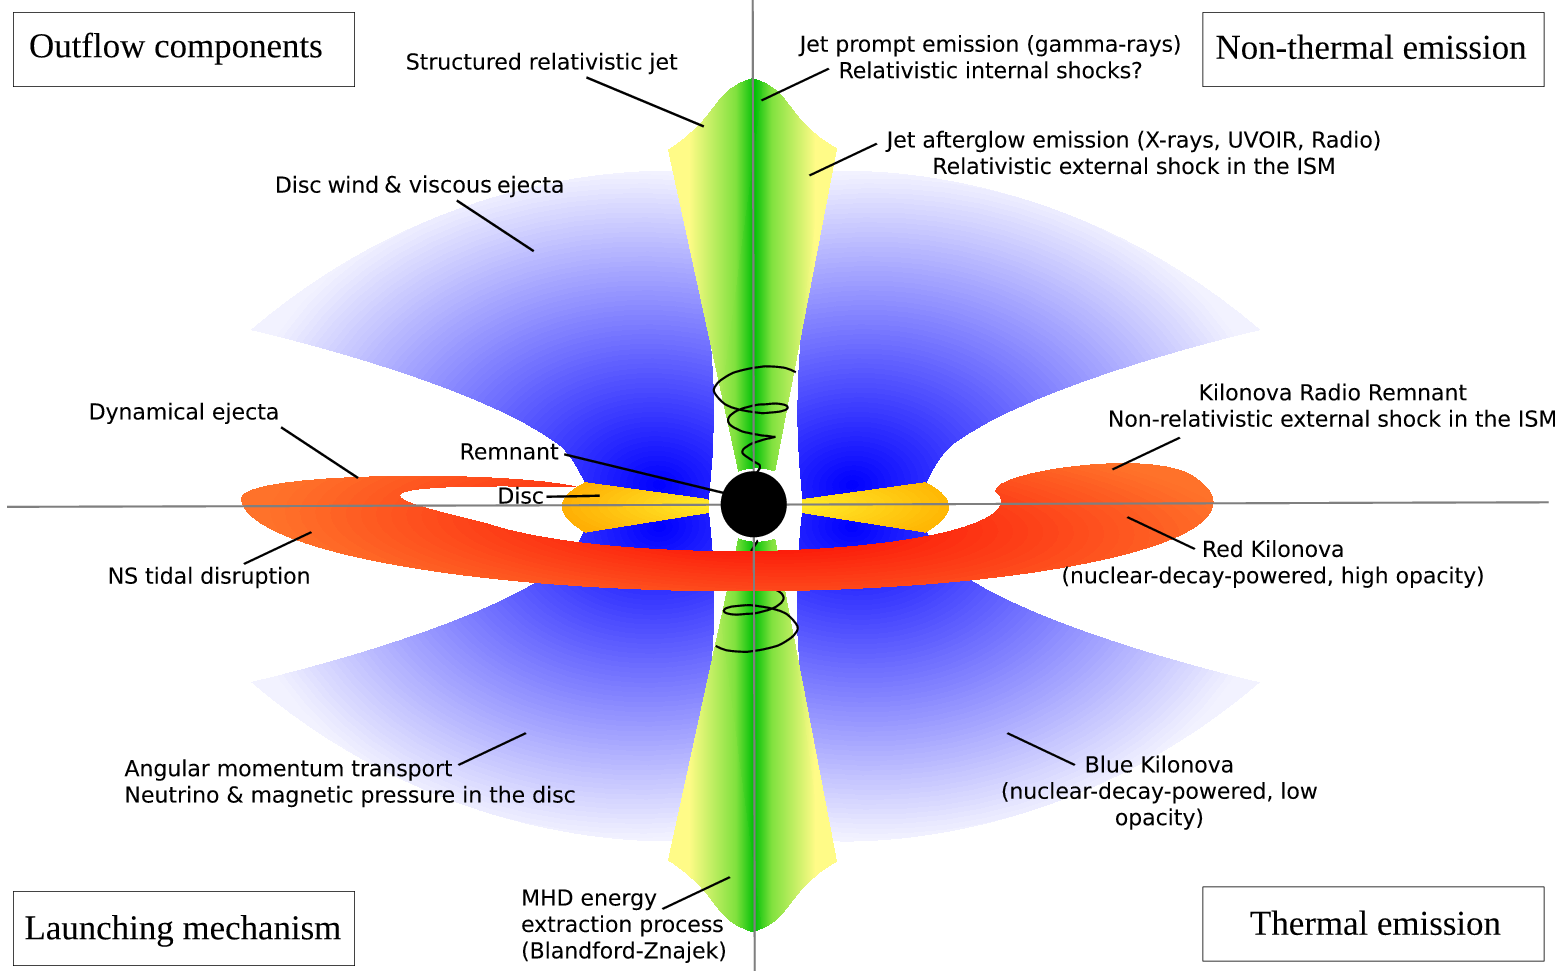
\includegraphics[width=\linewidth]{nsbh_outflows}
            \caption[EM outflows from NSBH mergers, from \cite{barbieri_2019a}]
            {
                Schematic diagram showing the various possible outflows from a suitable
                NSBH merger, along with their windows of visibility in the EM spectrum,
                their physical properties and their relevant launching/energy production
                mechanisms. From \cite{barbieri_2019a}.
            }
            \label{fig:nsbh_outflows}
        \end{figure}

        In order to better understand this event, an analysis similar to that in
        \S\S\ref{ssec:nsbh_190426} was carried out. The LSC data release for GW170817
        (part of the GWTC-1 catalog data release; see \cite{gwtc1_DR}) was used from
        which the binary system parameters were extracted. Note that for this data
        release, there are two `flavours' of posterior distributions which are supplied
        by the LSC data product, classified by the spin priors using in the Bayesian
        parameter estimation process.  The first is termed
        \texttt{IMRPhenomPv2NRT\_highSpin\_posterior}\footnote
        {
            \texttt{IMRPhenomPv2NRT} is the LAL C routine that models the
            phenomenological inspiral-merger-ringdown GW waveform for a spinning,
            precessing binary with numerical relativity-tuned tidal effects (see
            \cite{lalsuite}).
        }
        whereas the second is termed \texttt{IMRPhenomPv2NRT\_lowSpin\_posterior}, and
        both are considered in the current analysis.\\
        With the assumption that the heavier mass is the BH and the lighter mass the
        NS, the mass ratios, corresponding spins and tidal deformabilities are extracted
        from the posterior samples.  This was used to compute the $M_{disc}$
        corresponding to each set of samples, and the results for each flavour of
        the posterior distribution is shown below in Figs. \ref{fig:170817_low} --
        \ref{fig:170817_high}.

        \begin{figure}[ht]
            \centering
            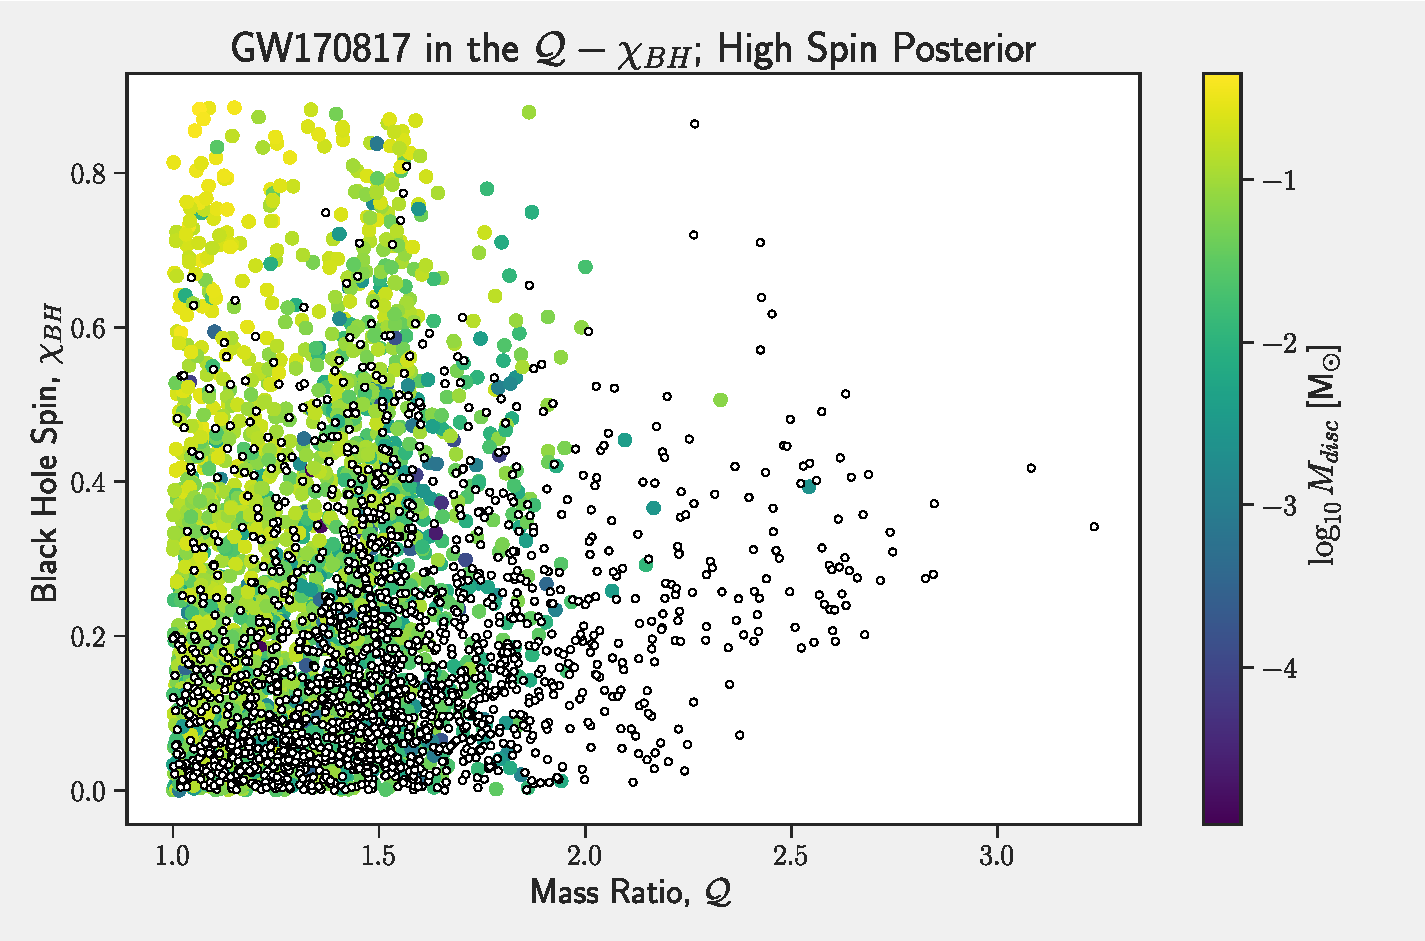
\includegraphics[width=\linewidth]{170817_in_q-chi-high}
            \caption[$M_{disc}$ for GW170817's High Spin Posterior Distribution]
            {
                Samples from the high spin posterior distribution for GW170817, in the
                $\mathcal{Q}-\chi_{BH}$ plane. The color coding for a point in the plane
                is the $M_{disc}$ computed for that $\mathcal{Q}$ and $\chi_{BH}$, and
                unfilled (white) circles represent posterior samples which have
                $M_{disc} = 0$.
            }
            \label{fig:170817_high}
        \end{figure}

        \begin{figure}[ht]
            \centering
            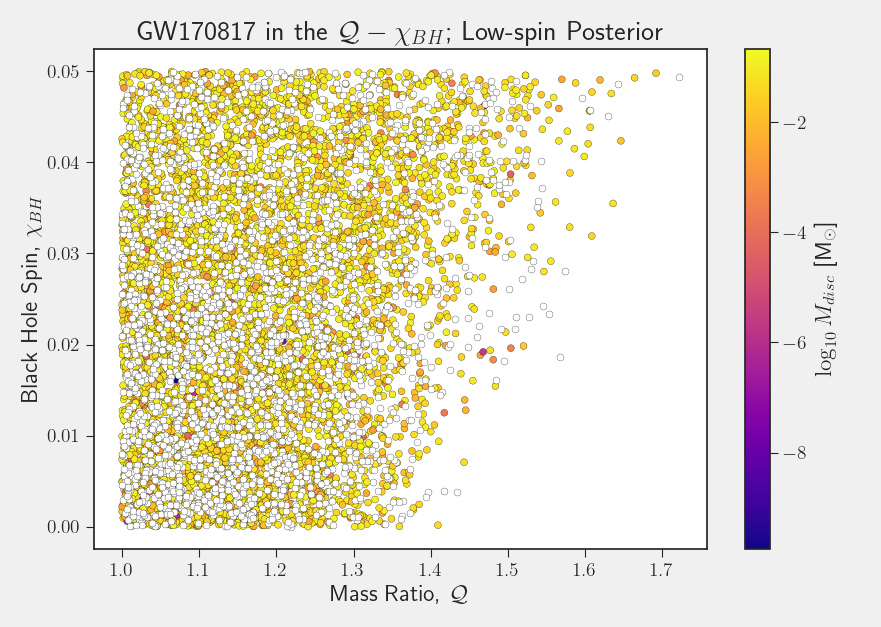
\includegraphics[width=\linewidth]{170817_in_q-chi-low}
            \caption[$M_{disc}$ for GW170817's Low Spin Posterior Distribution]
            {
                Samples from the low spin posterior distribution for GW170817, in the
                $\mathcal{Q}-\chi_{BH}$ plane. The color coding for a point in the plane
                is computed similar to the process followed in Fig.
                \ref{fig:170817_high}.
            }
            \label{fig:170817_low}
        \end{figure}

\section{Summary}
